\documentclass[a4paper, 10pt]{article}
\usepackage{pgf}
\usepackage{eurosym}
\usepackage{graphicx}
\usepackage{wasysym}
\usepackage{hyperref}
\usepackage{listings}
\usepackage{pxfonts}
\usepackage{verbatim}
\usepackage{color}
\usepackage{xcolor}
\usepackage{wrapfig}
\usepackage{enumitem}
\usepackage{booktabs}
\usepackage{tabularx}

\hypersetup{
    bookmarks=true,         % show bookmarks bar?
    unicode=true,          % non-Latin characters in Acrobat’s bookmarks
    pdftoolbar=true,        % show Acrobat’s toolbar?
    pdfmenubar=true,        % show Acrobat’s menu?
    pdffitwindow=true,     % window fit to page when opened
    pdftitle={Assignment 2},    % title
    pdfauthor={Paul Vesey},     % author
    pdfsubject={Construction Project Management},   % subject of the document
    pdfcreator={},   % creator of the document
    pdfproducer={xelatex}, % producer of the document
    pdfkeywords={'Project Management' }, % list of keywords
    pdfnewwindow=true,      % links in new PDF window
    colorlinks=true,       % false: boxed links; true: colored links
    linkcolor=violet,          % color of internal links (change box color with linkbordercolor)
    citecolor=magenta,        % color of links to bibliography
    filecolor=red,      % color of file links
    urlcolor=blue           % color of external links
}

\setlength\parindent{0pt}
\begin{document}

\lstset{language=HTML,
				basicstyle=\small,
				breaklines=true,
        numbers=left,
        numberstyle=\tiny,
        showstringspaces=false,
        aboveskip=-20pt,
        frame=leftline
        }
				
\begin{table}%
	\begin{minipage}{0.4\textwidth}%
			
\includegraphics[width=1\textwidth]{./img/LITlogo.jpg}
	\end{minipage}
	\qquad
	\centering
	\parbox{0.4\textwidth}{
		\begin{large}			
			\begin{tabular}{| r | l |} \hline
				Subject: & \textbf{Construction Project Management}\\
				Course: & \textbf{CPM Special Purpose Award}\\	
				Session: & \textbf{Spring 2020}\\
				Lecturer: & \textbf{Paul Vesey \footnotesize{BEng, MIE, HDip}}\\
				\hline
			\end{tabular}
		\end{large}			
	}
\end{table}
\vspace{0.25cm}	
	

\part*{Assignment 3 (35\%)- Project Management Documentation}


\begin{tabularx}{\textwidth}{ |X|X| }
	\hline
	\textbf{Issue Date:} & 27$^{th}$ November 2021\\
	\hline 
	\textbf{Submission Date:}  & 7$^{th}$ May 2022\\
	\hline
\end{tabularx}

\section*{Introduction}

This assignment will examine the following learning outcomes:\\

\begin{tabularx}{\textwidth}{ |c|X|c| }
	\hline
	\textbf{No.} & \textbf{Learning Outcome} & \textbf{Assessed} \\
	\hline 
	1  & Function as a project manager on a civil engineering project from project inception to completion. & Yes \\
	2  & Manage a project team and evaluate team performance. & Yes \\
	3  & Demonstrate and apply the concepts, techniques and skills in all ten knowledge areas of project management to construction and civil engineering projects. & Yes \\
	4  & Assess project risk and take appropriate mitigation measures. & Yes \\
	5  & Demonstrate skill and competence with current generation BIM project management tools. & Yes \\
	\hline
\end{tabularx}
\vspace{0.5cm}


This is an individual project.  You are encouraged to discuss your project with your peers, however all work submitted must be your own, with attribution where appropriate.\\

In this assignment you will create a detailed project plan for a construction project of your choice.  The project plan should include the traditional project management documents as well as a Post Contract Award BIM Execution Plan.  You are free to use the documentation pack used for Assignment 2.\\

The key deliverables for this project are:

\begin{enumerate}
	\item Detailed Project Management Plan as detailed.
	\item Post Contract BIM Execution Plan
\end{enumerate}


\section{Scenario}

Select a project with which you are familiar. The project must be a construction related project where BIM was or could be deployed.  The project must have at least 20 tasks and a maximum of 30, excluding heading items.\\

Develop the following items as detailed below. Descriptions of items \ref{sect:Scope} to \ref{sect:ReflectiveStatement} are available in the lecture notes, and are based on PMI's Project Management Body of Knowledge\\

You are to use the RIAI Template for Item \ref{sect:BEP}, the Post Contract BIM Execution Plan, available in the asset pack for this assignment.\\

The objective of this assignment is to produce a comprehensive project plan. The text of the document should clearly show how the various aspects of the project are going to be managed and controlled. You are encouraged to use appropriate standard templates and methodologies.  Standard Templates and Methodologies should be correctly attributed.\\

Your final document should be of professional standard in terms of content, layout and completeness. In essence, the completed document should be suitable for presentation to a prospective client.\\

The Reflective Statement should detail your learning experience while undertaking this coursework and your opinion on its relevance to the subject, etc.\\

You are encouraged to use Microsoft Project, Autodesk Revit, Autodesk Construction Cloud and other applications as appropriate.\\

This is a practical assignment. Your project management document should fully based on the practical implementation of project management theory.\\

\subsection{Project Scope Statement}\label{sect:Scope}
Your project scope statement should clearly describe your project and the key deliverables and constraints.  You are advised to examine various templates and generate your scope statement based on your research. 
\subsection{Work Breakdown Structure}
You may use Microsoft Project to create your work breakdown structure. You should have a maximum of 30 items, excluding items used for headings and groupings.  Items of work that are subcontracted do not have to be developed further down the WBS.
\subsection{Resource Breakdown Structure}
You are may select and use the most appropriate RBS structure for your project.  The structure does not need to be developed below subcontractor level.
\subsection{RACI Responsibility Assignment Matrix}
Your RACI matrix must be aligned with your WBS and RBS.  The use of Excel is advised for this section of the assignment. 
\subsection{Network Diagram, Gantt Charts and PERT Analysis}
Your WBS should form the basis for your Gantt Chart and Network Diagram.  Both of these elements must be generated in Microsoft Project.  The PERT analysis should be carried out in Excel, using the Critical Activities and Critical Path generated in Microsoft Project.  You will have to generate appropriate values for T$_{p}$ and T$_{o}$ in order to conduct this analysis.  Your report should include all calculations and workings, and show completion dates with 50\%, 85\% and 95\% probability.     


\subsection{Risk Management Plan}
Your Risk Management Plan should document the Risk Management processes that you are putting in place for this project.  The Risk Register should show the risks identified and the measures taken to manage these risks.  The timing of the risk events should coincide with the schedule for the project.


\subsection{Cost Management Plan}
Your Cost Management Plan should present a high level overview of the costs projections for the project, including the total overall value of the project, the proportion of the contract allocated to the main contractor and the value of subcontracted elements.  A time-based cost profile of the project should be included along with forecast modelling to determine the value and time of peak-debt.  You are also tasked with creating an three EVM tables for the project at key points in the project execution.  You will have to estimate your own percentage completion data based to complete this task.  Key items to be included in the report include EV, PV, \% complete, CPI, SPI, EAC and ETC for each time point.

\subsection{Communications Plan}

Provide a listing of the key stakeholders identified for the project.  Stakeholders should be categorised into 'Internal', 'External', 'Positive' and 'Negative'.  You are also required to generate an information distribution plan, complete with communication type and frequency.  A performance report requirements document is required for internal management stakeholders also.

\subsection{Human Resource Plan}

Your HR Plan should include details of the Project Team Requirements and the timing of the aquisation of those team members.  In each case you are to define the release criteria for these resources.  The data for this element should be consistant with the WBS, Procurement Plan, project schedule, and other elements.

\subsection{Procurement Management Plan} 

Provide an outline of an appropriate seller selection procedure to be used for this project.  This should clearly detail how sellers will be identified, shortlisted and selected.  Itendify 3 vital elements of the project that need to be sources from outside the organisation.  For these three elements provide details of the contract type and scope for each contract.

\subsection{Post Contract BIM Execution Plan}\label{sect:BEP}

Use the RIAI Post Contract BIM Execution Plan template provided in the asset pack for this assignment.  References to PAS1192 should be replaced with ISO19650 as appropriate.  This template is to be completed in full, and should be consistent with all other elements in this assignment. 


\subsection{Reflective Statement}\label{sect:ReflectiveStatement} 

There are numerous reflective practice frameworks in common use.  The diagram shown at Figure \ref{fig:gibbs-diagram} depicts the Gibbs Reflective Cycle.  Use this framework to reflect on your learning.


\begin{figure}[h!]
	\centering
	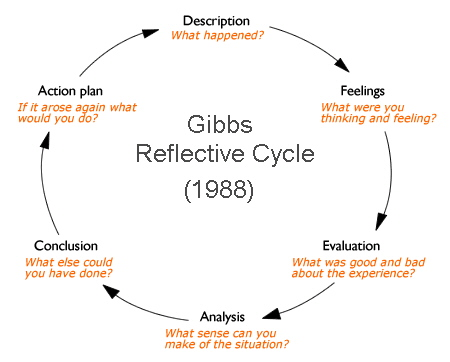
\includegraphics[width=0.7\linewidth]{img/gibbs-diagram}
	\caption{Gibbs Reflective Cycle}
	\label{fig:gibbs-diagram}
\end{figure}



\newpage
\section{Submission Details \& Marking Scheme}


\subsection{Late Submission}
Failure to submit your assignment on or before the date and time indicated on MS Teams will result in a penalty of 5\% per day or part thereof.

\subsection{Marking Scheme}

\begin{tabularx}{\textwidth}{ |c|X|l|c| }
		\hline
		\textbf{Item} & \textbf{Description} & \textbf{Max Required} & \textbf{Mark} \\
		\hline
		\hline
		1  & Project Scope Statement &  2 pages  & 10\% \\
		\hline
		2  & Work Breakdown Structure &  30 elements  & 5\% \\
		\hline
		3  & Resource Breakdown Structure &  15 elements  & 5\% \\
		\hline
		4  & RACI Responsibility Assignment Matrix &  A3 Diagram  & 5\% \\
		\hline
		5  & Network Diagram, Gantt Charts and PERT Analysis &  A3 Diagrams  & 5\% \\
		\hline
		6  & Risk Management Plan & 2 pages  & 10\% \\
		&	- Methodology  & & \\
		&	- Timing of Risk Events  & & \\
		&	- Risk Register  & & \\
		\hline
		7  & Cost Control Plan &  2 pages  & 5\% \\
		&	- Total value of contract  & & \\
		&	- Proportion to contractor  & & \\
		&	- Proportion subcontracted   & & \\
		&	- Project Cash Flow Profile and Peak Debt  & & \\
		&	- EVM Table for 3 key time-points  & & \\
		\hline
		8  & Communications Plan &  2 pages  & 5\% \\
		&	- Identified Stakeholders  & & \\
		&	- Information Distribution Plan  & & \\
		&	- Performance Report Requirements  & & \\
		\hline
		9  & Human Resource Plan &  1 page  & 10\% \\
		&	- Project Team Acquisition Plan & & \\
		&	- Release Criteria  & & \\
		\hline
		10  & Procurement Management Plan &  1 page  & 5\% \\
		&	- Seller Selection Procedure  & & \\
		&	- Identify 3 vital project elements that need to be sourced from outside the organisation.  Allocate contract types to each of these.  & & \\
		\hline
		11  & Post Contract BIM Execution Plan &  as per template  & 30\% \\
		\hline
		12  & Reflective Statement &  1 page  & 5\% \\
		\hline
		\hline
		& & \textbf{Total} & \textbf{100\%} \\
		\hline
\end{tabularx}




\newpage
\subsection*{Submission Checklist}

All files are to be submitted.  Do not submit links to shared files or folders as these may not be accessible for grading.  Ensure that you 'Turn In' your assignment on Teams.  \textbf{It is not enough to upload your submission files; you must turn in your work}.\\

A single pdf file is required for all of the elements listed above.  You must also include a single zip file containing all of the source files used, such as Microsoft Project, Word, Excel, etc.  Do not use any other compression/archiving technology such as 7-Zip or WinRAR.\\

Your submission should contain a cover page, table of contents, references and appendices as appropriate.\\

Your Word document should transition from A4 to A3 paper, Portrait/Landscape orinetaion as needed to present the information required.\\

All files to follow PAS file naming convention as per the BEP.  In general this will be of the format \textit{PMBM03-***-00-ZZ-**-A1-P01}, where *** is to be replaced by the last 3 digits of your K-number and ** indicates the document type as stated in your BEP.\\

Complete and include the following checklist table in your submission.  Provide multiple filenames for each Item as appropriate. \\


\begin{tabularx}{\textwidth}{ |c|X|l| }
	\hline
	\textbf{Item} & \textbf{Description} & \textbf{Filename(s)} \\
	\hline
	\hline
	1  & Project Scope Statement & \\
	\hline
	2  & Work Breakdown Structure & \\
	\hline
	3  & Resource Breakdown Structure & \\
	\hline
	4  & RACI Responsibility Assignment Matrix &  \\
	\hline
	5  & Network Diagram, Gantt Charts and PERT Analysis &  \\
	\hline
	6  & Risk Management Plan & \\
	\hline
	7  & Cost Control Plan &  \\
	\hline
	8  & Communications Plan & \\
	\hline
	9  & Human Resource Plan &  \\
	\hline
	10  & Procurement Management Plan & \\
	\hline
	11  & Post Contract BIM Execution Plan &   \\
	\hline
	12  & Reflective Statement & \\
	\hline
\end{tabularx}

\end{document}